% !TeX document-id = {4c50d318-ae06-42ec-8e3f-7706d393a431}
% !TeX spellcheck = sl_SI
% !TeX program = pdflatex+bibtex+makeindex
% vim: set spell spelllang=sl:
% za preverjanje črkovanja, če se uporablja Texstudio ali vim
\documentclass[12pt,a4paper,twoside]{article}
\usepackage[utf8]{inputenc}  % pravilno razpoznavanje unicode znakov

% NASLEDNJE UKAZE USTREZNO POPRAVI
\newcommand{\program}{Matematika} % ime studijskega programa
\newcommand{\imeavtorja}{Gašper Domen Romih} % ime avtorja
\newcommand{\imementorja}{prof.~dr.~Nino Bašić} % akademski naziv in ime mentorja, uporabi poln naziv, prof.~dr.~, doc.~dr., ali izr.~prof.~dr.
\newcommand{\imesomentorja}{} % akademski naziv in ime somentorja, če ga imate
\newcommand{\naslovdela}{1-2-3 Domneva}
\newcommand{\letnica}{2020} % letnica magistriranja
\newcommand{\opis}{Delo obravnava 1-2-3 domnevo ter njene variacije.}  % Opis dela v eni povedi. Ne sme vsebovati matematičnih simbolov v $ $.
\newcommand{\kljucnebesede}{teorija grafov\sep kombinatorika} % ključne besede, ločene z \sep, da se PDF metapodatki prav procesirajo
\newcommand{\keywords}{integration\sep complex} % ključne besede v angleščini
\newcommand{\organization}{Univerza v Ljubljani, Fakulteta za matematiko in fiziko} % fakulteta
\newcommand{\literatura}{literatura}  % pot do datoteke z literaturo (brez .bib končnice)
\newcommand{\sep}{, }  % separator med ključnimi besedami v besedilu
% KONEC PODATKOV

\usepackage{bibentry}         % za navajanje literature v programu dela s celim imenom
\nobibliography{\literatura}
\newcommand{\plancite}[1]{\item[\cite{#1}] \bibentry{#1}} % citiranje v programu dela

\usepackage{filecontents}  % za pisanje datoteke s PDF metapodatki
\usepackage{silence} \WarningFilter{latex}{Overwriting file}  % odstrani annoying warning o obstoju datoteke
% datoteka s PDF metapodatki, zgenerira se kot magisterij.xmpdata
\begin{filecontents*}{\jobname.xmpdata}
  \Title{\naslovdela}
  \Author{\imeavtorja}
  \Keywords{\kljucnebesede}
  \Subject{\opis}
  \Org{\organization}
\end{filecontents*}

\usepackage[a-1b]{pdfx}  % zgenerira PDF v tem PDF/A-1b formatu, kot zahteva knjižnica
\hypersetup{bookmarksopen, bookmarksdepth=3, colorlinks=true,
  linkcolor=black, anchorcolor=black, citecolor=black, filecolor=black,
  menucolor=black, runcolor=black, urlcolor=black, pdfencoding=auto,
  breaklinks=true, psdextra}

\usepackage[slovene]{babel}  % slovenščina
\usepackage[T1]{fontenc}     % naprednejše kodiranje fonta
\usepackage{amsmath,amssymb,amsfonts,amsthm} % matematični paketi
\usepackage{graphicx}     % za slike
%\usepackage[dvipsnames,usenames]{color} % barve
\usepackage{emptypage}    % prazne strani so neoštevilčene, ampak so štete
\usepackage{units}        % fizikalne enote kot \unit[12]{kg} z polovico nedeljivega presledka, glej primer v kodi
\usepackage{makeidx}      % za stvarno kazalo, lahko zakomentiraš, če ne rabiš
\makeindex                % za stvarno kazalo, lahko zakomentiraš, če ne rabiš
% oblika strani
\usepackage[
  top=3cm,
  bottom=3cm,
  inner=3.5cm,      % margini za dvostransko tiskanje
  outer=2.5cm,
  footskip=40pt     % pozicija številke strani
]{geometry}

% VEČ ZANIMIVIH PAKETOV
% \usepackage{array}      % več možnosti za tabele
% \usepackage[list=true,listformat=simple]{subcaption}  % več kot ena slika na figure, omogoči slika 1a, slika 1b
% \usepackage[all]{xy}    % diagrami
% \usepackage{doi}        % za clickable DOI entrye v bibliografiji
% \usepackage{enumerate}     % več možnosti za sezname

% Za barvanje source kode
% \usepackage{minted}
% \renewcommand\listingscaption{Program}

% Za pisanje psevdokode
% \usepackage{algpseudocode}  % za psevdokodo
% \usepackage{algorithm}
% \floatname{algorithm}{Algoritem}
% \renewcommand{\listalgorithmname}{Kazalo algoritmov}

% DRUGI TVOJI PAKETI:
% tukaj
\usepackage{tikz}
\usetikzlibrary{quotes} % LATEX and plain TEX
\usetikzlibrary{arrows,automata,positioning}

\usetikzlibrary{shapes.geometric}
\usepackage{subcaption}
\usepackage{mwe}
\usepackage{float}


\setlength{\overfullrule}{50pt} % označi predlogo vrstico
\pagestyle{plain}               % samo številka strani na dnu, nobene glave / noge

% ukazi za matematična okolja
\theoremstyle{definition} % tekst napisan pokončno
\newtheorem{definicija}{Definicija}[section]
\newtheorem{primer}[definicija]{Primer}
\newtheorem{opomba}[definicija]{Opomba}
\newtheorem{aksiom}{Aksiom}
\newtheorem{domneva}[definicija]{Domneva}

\theoremstyle{plain} % tekst napisan poševno
\newtheorem{lema}[definicija]{Lema}
\newtheorem{izrek}[definicija]{Izrek}
\newtheorem{trditev}[definicija]{Trditev}
\newtheorem{posledica}[definicija]{Posledica}


\numberwithin{equation}{section}  % števec za enačbe zgleda kot (2.7) in se resetira v vsakem poglavju

% Matematični ukazi
\newcommand{\R}{\mathbb R}
\newcommand{\N}{\mathbb N}
\newcommand{\Z}{\mathbb Z}
\renewcommand{\C}{\mathbb C}
\newcommand{\Q}{\mathbb Q}

% \DeclareMathOperator{\tr}{tr}  % morda potrebuješ operator za sled ali kaj drugega?

% bold matematika znotraj \textbf{ }, tudi v naslovih, kot \omega spodaj
\makeatletter \g@addto@macro\bfseries{\boldmath} \makeatother

% Poimenuj kazalo slik kot ``Kazalo slik'' in ne ``Slike''
\addto\captionsslovene{
  \renewcommand{\listfigurename}{Kazalo slik}%
}

% če želiš, da se poglavja začnejo na lihih straneh zgoraj
% \let\oldsection\section
% \def\section{\cleardoublepage\oldsection}

%%%%%%%%%%%%%%%%%%%%%%%%%%%%%%%%%%%%%%%%%%
%%%%%%           DOCUMENT           %%%%%%
%%%%%%%%%%%%%%%%%%%%%%%%%%%%%%%%%%%%%%%%%%

\begin{document}

\pagenumbering{roman} % začnemo z rimskimi številkami
\thispagestyle{empty} % ampak na prvi strani ni številke

\noindent{\large
UNIVERZA V LJUBLJANI\\[1mm]
FAKULTETA ZA MATEMATIKO IN FIZIKO\\[5mm]
\program\ -- 2.~stopnja}
% ustrezno dopolni za IŠRM
\vfill

\begin{center}
  \large
  \imeavtorja\\[3mm]
  \Large
  \textbf{\MakeUppercase{\naslovdela}}\\[10mm]
  \large
  Magistrsko delo \\[1cm]
  Mentor: \imementorja \\[2mm] % ustrezno popravi spol
%   Somentor: \imesomentorja   % dodaj, če potrebno
\end{center}
\vfill

\noindent{\large Ljubljana, \letnica}

\cleardoublepage

%% IZJAVA O AVTORSTVU
%\pdfbookmark[1]{Izjava o avtorstvu}{izjava} % bookmark v PDF, \pdfbookmark[nivo]{text}{label}
%
%% izjava: po potrebi spremeni v žensko obliko
%\setlength\topsep{0pt}
%\setlength\parskip{0pt}
%\begin{center}
%  \textbf{Univerza v Ljubljani} \\
%  \textbf{Fakulteta za matematiko in fiziko}
%
%  \vfill
%
%  \underline{Izjava o avtorstvu, istovetnosti tiskane in elektronske verzije magistrskega dela in} \\
%  \underline{objavi osebnih podatkov študenta}
%
%  \vfill
%
%  \setlength\topsep{0pt}
%  \setlength\parskip{0pt}
%  \begin{flushleft}
%    Spodaj podpisani študent \imeavtorja{} avtor magistrskega dela (v nadaljevanju: pisnega
%    zaključnega dela študija) z naslovom:
%  \end{flushleft}
%
%  \vfill
%
%  \textbf{\naslovdela}
%
%  \vfill
%
%  IZJAVLJAM
%\end{center}
%
%\begin{enumerate}[1. ]
%  \item \emph{Obkrožite eno od variant a) ali b)}
%  \begin{enumerate}[a)]
%    \item da sem pisno zaključno delo študija izdelal samostojno;
%    \item da je pisno zaključno delo študija rezultat lastnega dela več kandidatov in izpolnjuje
%      pogoje, ki jih Statut UL določa za skupna zaključna dela študija ter je v zahtevanem deležu
%      rezultat mojega samostojnega dela;
%  \end{enumerate}
%  pod mentorstvom IZPOLNI. % dopiši \imementorja v rodilniku
%%   \\ in somentorstvom IZPOLNI. % dopiši \imesomentorja v rodilniku
%  \item da je tiskana oblika pisnega zaključnega dela študija istovetna elektronski obliki
%    pisnega zaključnega dela študija;
%  \item da sem pridobil vsa potrebna dovoljenja za uporabo podatkov in avtorskih del v pisnem
%    zaključnem delu študija in jih v pisnem zaključnem delu študija jasno označil;
%  \item da sem pri pripravi pisnega zaključnega dela študija ravnal v skladu z etičnimi načeli in,
%    kjer je to potrebno, za raziskavo pridobil soglasje etične komisije;
%  \item da soglašam, da se elektronska oblika pisnega zaključnega dela študija uporabi za preverjanje
%    podobnosti vsebine z drugimi deli s programsko  opremo za preverjanje podobnosti
%    vsebine, ki je povezana s študijskim informacijskim sistemom fakultete;
%  \item da na UL neodplačno, neizključno, prostorsko in časovno neomejeno prenašam pravico shranitve
%    avtorskega dela v elektronski obliki, pravico reproduciranja ter pravico dajanja pisnega
%    zaključnega dela študija na voljo javnosti na svetovnem spletu preko Repozitorija UL;
%  \item da dovoljujem objavo svojih osebnih podatkov, ki so navedeni v pisnem zaključnem delu študija
%    in tej izjavi, skupaj z objavo pisnega zaključnega dela študija.
%\end{enumerate}
%
%\vfill
%
%\noindent
%Kraj:  \hfill   Podpis študenta: \phantom{prostor za podpis}
%
%\vfill
%
%\noindent
%Datum:
%
%\cleardoublepage
%% END IZJAVA O AVTORSTVU

% zahvala
\pdfbookmark[1]{Zahvala}{zahvala} %
\section*{Zahvala}
Neobvezno.
Zahvaljujem se \dots
% end zahvala -- izbriši vse med zahvala in end zahvala, če je ne rabiš

\cleardoublepage

\pdfbookmark[1]{\contentsname}{kazalo-vsebine}
\tableofcontents

% list of figures
% \cleardoublepage
% \pdfbookmark[1]{\listfigurename}{kazalo-slik}
% \listoffigures
% end list of figures

\cleardoublepage

\section*{Program dela}
\addcontentsline{toc}{section}{Program dela} % dodajmo v kazalo
Tu naj bi mentor napisal program dela, skupaj z osnovno literaturo spodaj. To je v template-u, ki ga iamo na spletni učilnici za seminar. Verjetno tega ni v končno verziji. Okviren osnutek z povezavami na določene reference bom napisal kar v glavnem delu dokumenta.

\section*{Osnovna literatura}
Literatura mora biti tukaj posebej samostojno navedena (po pomembnosti) in ne
le citirana. V tem razdelku literature ne oštevilčimo po svoje, ampak uporabljamo
okolje itemize in ukaz plancite, saj je celotna literatura oštevilčena na koncu.
\begin{itemize}
  \plancite{maingraph}
  \plancite{base}
  \plancite{regularWeightening}
  \plancite{kncoloring}
  \plancite{weigheting12345}
\end{itemize}

\vspace{2cm}
\hspace*{\fill} Podpis mentorja: \phantom{prostor za podpis}

% \vspace{2cm}
% \hspace*{\fill} Podpis somentorja: \phantom{prostor za podpis}

\cleardoublepage
\pdfbookmark[1]{Povzetek}{abstract}

\begin{center}
\textbf{\naslovdela} \\[3mm]
\textsc{Povzetek} \\[2mm]
\end{center}
Povezavam grafa $G$ priredimo uteži z vrednostmi $1,2,\ldots,k$. Uteži na povezavah porodijo pravilno barvanje grafa $G$, če se vsote uteži incedenčnih povezav razlikujejo za vsaki sosednji vozlišči. V nalogi se osredotočimo na zgornjo mejo za $k$ za splošne grafe. Obravnavamo tudi polne ter $d$-regularne grafe. 

\vfill
\begin{center}
\textbf{English translation of the title} \\[3mm] % prevod slovenskega naslova dela
\textsc{Abstract}\\[2mm]
\end{center}

An abstract of the work is written here. This includes a short description of
the content and not the structure of your work.

\vfill\noindent
\textbf{Math.~Subj.~Class.~(2010):} oznake kot 74B05, 65N99, na voljo so na naslovu
\url{http://www.ams.org/msc/msc2010.html?t=65Mxx} \\[1mm]
\textbf{Ključne besede:} \kljucnebesede \\[1mm]
\textbf{Keywords:} \keywords

\cleardoublepage

\setcounter{page}{1}    % od sedaj naprej začni zopet z 1
\pagenumbering{arabic}  % in z arabskimi številkami

\section{Uvod}
Napišite kratek zgodovinski in matematični uvod.  Pojasnite motivacijo za problem, kje
nastopa, kje vse je bil obravnavan. Na koncu opišite tudi organizacijo dela -- kaj je v kakšnem
razdelku.

\section{Osnovne definicije in pojmi}

V tem razdelku na kratko predstavim grafe ter naveden definicije, ki bodo potrebne kaseje v nalogi. Pri tem mislim predvsem na barvanje, prirejanje, polni grafi, regularni grafi, itd. Večina definicij bi povzel po~\cite{maingraph}, kar je bila tudi glavna referenca pri predmetu teorija grafov.

Graf bomo označili kot urejn par $G=(V, E)$. Pri tem množico $V$ imenujemo množica vozlišč grafa in njene elemente ponavadi označimo z $u, v, w$. Množica $E \subset V \times V$ je množica povezav grafa $G$. Njene elemente ponavadi označujemo z $e, f, g$ kadar nas ne zanima kateri dve vozlišči povezava vsebuje. V nasprotnem primeru povezavo označimo z $uv \in E$ in s tem eksplicitno povemo, da je to potem povezava med vozliščem $v$ in $u$. Množico vozlišč in povezav grafa, lahko zaporedoma označimo tudi kot $V(G)$ in $E(G)$. V izogib težavam z notacijo bomo vedno predpostavili, da $V \cap E = \emptyset$. 
\begin{primer}
	Vzemimo graf $$G = (\{1,2,3,4,5,6\}, \{\{1,2\}, \{1,5\}, \{2,5\}, \{5,4\}, \{2,3\}, \{4,3\}, \{4,5\}, \{4,6\}\}).$$ 
	
	Potem ena izmed možnih risb grafa izgleda takole:
	
	\begin{tikzpicture}
	[scale=.8,auto=left,every node/.style={circle,draw=black,fill=white!20}]
	\node (n6) at (1,10) {6};
	\node (n4) at (4,8)  {4};
	\node (n5) at (8,9)  {5};
	\node (n1) at (11,8) {1};
	\node (n2) at (9,6)  {2};
	\node (n3) at (5,5)  {3};
	
	\foreach \from/\to in {n6/n4,n4/n5,n5/n1,n1/n2,n2/n5,n2/n3,n3/n4}
	\draw (\from) -- (\to);
	
	\end{tikzpicture}
\end{primer}
Za $v \in V(G)$ lahko definiramo t.i. odprto soseščino vozlišča $N(v)$. To je množica vseh sosedov vozlišča $u$, torej $N(v) = \{u \in V(G) \mid uv \in E(G), u \neq v \}$. Na enak način definiramo zaprto soseščino vozlišča $N\left[u\right] = N(v) \cup \{v\}$. Poleg množice sosedov je pomembna tudi njena moč, kar označimo z $d(v)$ in imenujemo stopnja vozlišča $v$.

\section{Barvanje grafa in uteži na povezavah}

V tem razdelku bi predstavil idejo 1-2-3 domneve. Tore kako pridemo iz uteženega grafa do barvanja ter argumentiram zakaj lahko pridemo do pravilnega barvanja, če nimamo omejitev na množici uteži. Na tem mestu bi tudi predstavil domnevo, povzeto po~\cite{base}.
Nekako bo tudi treba poimenovati engleški term 'edge weighting graph coloring'. Za sedaj bom temu rekel barvanje grafa z uteženimi povezavami.
\subsection{Barvanje grafa}
Vozliščno barvanje grafa $G=(V, E)$ je preslikava $ c: V \rightarrow S$, za katero velja $c(v) \neq c(u)$, če $vu \in E$. Množica $S$ je množica razpoložljivih barv. Poleg vozliščnega barvanja poznamo tudi povezavno barvanje, vendar nas to tekom magisterske naloge nebo zanimalo. Zato bomo od sedaj dalje z barvanjem grafa vedno mislili vozliščno barvanje. Pri barvanju nas ponavadi predvsem zanima velikost množice $S$. Drugače povedano, zanima nas najmanjši $k \in \mathbb{N}$, tako da G premore $k$-barvanje $c : V \rightarrow \{1,2,\ldots, k\}$. Tak najmanjši $k$ označimo z $\chi(G)$ in ga imenujemo kromatično število grafa $G$. V kolikor je $ \chi(G) \le k$ rečemo, da je graf $k$-obarljiv.

\subsection{Uteženi grafi}
Povezavam grafa velikokrat priredimo t.i. uteži, ponavadi iz množice pozitivnih realnih števil. Take utežitve grafa imajo v praksi veliko uporabnost. Poleg tega, da uteži priredimo povezavam, lahko uteži priredimo tudi vozliščem. z namenom, da bomo ločili med rezličnimi utežitvami grafa, definirajmo povezavno utežitev kot preslikavo $\omega : E(G) \rightarrow S$. Na podoben način definiramo vozliščno utežitev kot preslikavo $\omega : V(G) \rightarrow S$. V kolikor graf utežimo tako povezavno kot vozliščno rečemo, da imamo polno utežitev grafa $G$. V našem primeru bo množica uteži $S$ vedno končna množica prvih $k$ naravnih števil, kar lahko označimo kot $S = \left[k\right] = \{1,2, \ldots, k\}$. S pomočjo zgornjih dejstev lahko definiramo naslednjo definicijo.
\begin{definicija}
	 Definiramo \textbf{$k$-utežitev} grafa $G$ kot preslikavo 
	 $$ \omega : D \rightarrow {1,2,\ldots, k},$$
	 kjer za množico $D$ vzamemo $E(G)$, $V(G)$ ali $V(G) \cup E(G)$.
\end{definicija}

\subsection{Barvanje grafa z utežmi}
V prejšnem razdelku smo definirali pojem $k$-uteženega grafa. Hitro lahko vidimo, da nam $k$-utežitev $\omega$ lahko inducira neko barvanje grafa $G$, tako da za barvo nekega vozlišča $v$ vzamemo vsoto uteži na povezavah incidenčnih $v$. Označimo
$$ c_{\omega} (v) = \sum_{u \in N(v)} \omega(vu). $$
 V kolikor imamo polno utežitev, prištejemo še utež vozlišča $v$. Seveda se tu porodi vprašanje, ali je tako barvanje sploh pravilno, torej ali je izpolnjena zahteva, da sta sosednji vozlišči pobarvani različno. Hitro ugotovimo, da to ni možno za graf $K_2$, zato bomo v nadaljevanju predpostavljali, da je $G$ povezan graf, ki ni $K_2$. Prepričajmo se sedaj, da za vsak graf $G$ obstaja tak $k \in \mathbb{N}$, tako da obstaja $k$-utežitev grafa $G$, ki porodi pravilno barvanje. Še več pokazali bomo, da je vsako vozlišče različne barve. V ta namen označimo $\Delta = \Delta(G)$ maksimalno stopnjo in oštevilčimo povezave grafa $G$ kot $e_1, e_2, \ldots, e_m$, kjer je $m = |E(G)|$. Sedaj definiramo utežitev kot 
$$\omega(e_i) = \Delta ^i .$$
Očitno ta utežitev porodi pravilno barvanje grafa $G$. Vendar je zgornja ocena precej slaba ter predvsem različna za vsak graf.
\begin{definicija}
	Rečemo, da je $k$-utežitev $\omega$ grafa $G$  \textbf{pravilno barvanje z utežmi}, če za vsak $uv \in E(G)$ velja
	$$c_{\omega} (u) \neq c_{\omega}(v). $$
\end{definicija}
Označimo najmanjši tak $k$, da za graf $G$ obstaja $k$-utežitev, ki je pravilno barvanje z utežmi kot $\mu(G)$. Smiselno vprašanje na tem mestu bi bilo, ali obstaja zgornja meja za $\mu(G)$ za vsak povezan graf, ki ni $K_2$. Kot bomo videli v nadaljevanju je odgovor na to vprašanje pozitiven, zato je smiselno razmišljati o tem kako visoka je ta zgornja meja. Sedaj lahko navedemo domnevo, ki glavna tema te naloge.
\begin{domneva} 
	\label{123conjecture}
	(1-2-3 Domneva; Karonski– Luczak–Thomason~\cite{base}) Naj bo $G$ povezan graf, ki ni $K_2$. Tedaj je $\mu(G) \le 3.$ 
\end{domneva}
Za sedaj še niti vemo, ali obstaja fiksna zgornja meja za vsak graf. V članku ~\cite{base}, kjer je bila zastavljena zgornja domneva so pokazali, da obstaja končna množica realnih števil, tako da utežitev z temi števili inducira pravilno barvanje vsakega grafa. Vendar je ta rezultat še vedno precej odmaknjen od željene domneve. Kasneje je bil v ~\cite{weigheting12345} predstavljen eleganten algoritem, ki doseže zahtevano utežitev z utežmi v $\{1,2,3,4,5\}$. To je do sedaj tudi najboljši razultat za splošne grafe. Tekom naloge bomo spoznali nekaj metod s katerimi se lahko lotimo zgornjega problema za neke specifične družine grafov ter se probamo čim bolj približati željenemu rezultatu. Za začetek pa si oglejmo nekaj preprostih družin, za katere pokaže, da zgornja meja velja.
\begin{primer}[Izračun za grafe $P_n$]
	Ker je graf $P_2 = K_2$ bomo obravnavali le primer, ko je $n \ge 3$. Najprej oštevilčimo povezave $P_n$ na naraven način kot $e_i = v_i v_{i+1}$ za $i=1,2,\ldots, n-1$. Po kratkem premisleku ugotovimo, da je potreben pogoj za željeno utežitev
	$$\omega(e_i) \neq \omega(e_j) \text{ v kolikor } |j-i| = 2 .$$
	Torej povezavi, ki sta na razdalji $2$ morata imeti različne uteži. To drži, saj imata v primeru ko $\omega(e_i) = \omega(e_{i+2})$ vozlišči $v_{i+1}$ in $v_{i+2}$ enako barvo neglede na vrednost $\omega(e_{i+1})$. Polega tega, da je zgornji pogoj potreben, je tudi zadosten. To preprosto vidimo saj smo ugotovili, da povezava $e_{i}$ ne vpliva na barvo vozlišč $v_i$ in $v_{i+1}$ saj obema "pripomore" enako vrednost. Na podlagi zgornjega razmisleka ugotovimo, da $\mu(P_3) = 1$, saj $P_3$ ne vsebuje povezav na razdalji 2. Po drugi strani za $P_n$ definiramo:
	\begin{equation*}
	\omega(e_i) = \begin{cases}
			1 &i \equiv 1,2 \pmod{4}\\ 
			2 &i \equiv 3,4 \pmod{4}
	\end{cases}
	\end{equation*}
	
	\begin{figure}[!h]
		\centering
		\label{fig:pn}
		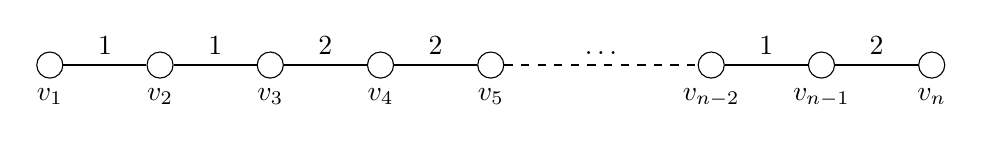
\begin{tikzpicture}
		[scale=.7,auto=left,main node/.style={shape=circle,draw,fill=white}]
		\node [main node] (1) at (1,1) [label=below:$v_1$] {} ;
		\node [main node](2) at (3,1) [label=below:$v_2$] {} ;
		\node [main node](3) at (5,1) [label=below:$v_3$] {} ;
		\node [main node](4) at (7,1) [label=below:$v_4$] {} ;
		\node [main node](5) at (9,1) [label=below:$v_5$] {} ;
		
		\node [main node](6) at (13,1) [label=below:$v_{n-2}$] {} ;
		\node [main node](7) at (15,1) [label=below:$v_{n-1}$] {} ;
		\node [main node](8) at (17,1) [label=below:$v_n$]  {};
		
		
		\path[draw,thick]
		(1) edge node {1} (2)
		(2) edge  node {1} (3)
		(3) edge  node {2} (4)
		(4) edge  node {2} (5)
		
		(5) edge [dashed]  node {$\ldots$} (6)
		
		(6) edge  node {1} (7)
		(7) edge  node {2} (8)
		;
		
		\end{tikzpicture}
		\caption{Primer utežitve grafa $P_n$.}
	\end{figure}
	Res, zgornja utežitev zadošča zgornjemu pogoju. Na sliki ~\ref{fig:pn} vidimo primer neke take utežitvne na grafu $P_n$. Glede na to, da sta zadnji uteži na povezavah $1$ in $2$ lahko sklepamo, da gre na sliki za $P_n$ z $n \equiv 3 \pmod{4}$. Prav tako opazimo, da je pravzaprav pomembno zaporednje uteži $11221\ldots 112$. V tem zaporedju se torej nujno razlikujeta elementa na razdalji 2. Tako lahko zaključimo, da je $\mu(P_n) = 2$ za $n \ge 4$. Podoben razmislem bomo uporabili v naslednjem primeru.
\end{primer}


\begin{primer}[Izračun za grafe $C_n$]
	
	V prejšnjem primeru smo izračunali število $\mu$ za grafe, ki so poti. Hitro opazimo, da med potjo in ciklom ni veliko razlike. Dodana je le ena povezava med prvim in zadnjim vozliščem. Enako kot v prejšnjem primeru bomo oštevilčili povezave cikla $C_n$ kot $e_1, e_2, \ldots, e_n$, kjer vzamemo $e_n = v_n v_1$. Poizkusimo z enako utežitvijo kot smo jo imeli za poti, torej
		\begin{equation*}
	\omega(e_i) = \begin{cases}
	1 &i \equiv 1,2 \pmod{4}\\ 
	2 &i \equiv 3,4 \pmod{4}
	\end{cases}
	\end{equation*}
	
\begin{figure}[H]
	\centering 
	\begin{subfigure}{0.475\textwidth}
		\centering 
		\begin{tikzpicture}
	
		[scale=.6,auto=left,main node/.style={draw=none,fill=none}]
		\def \n {7}
		\node[
		regular polygon,
		regular polygon sides=\n,
		minimum size=4cm,
		rotate=180/\n,
		] (a) {};
		
		\node[draw=none,fill=none] (1) at (a.corner 1) [] { $v_1$};
		\node[draw=none,fill=none] (2) at (a.corner 2) [] { $v_2$};
		\node[draw=none,fill=none] (3) at (a.corner 3) [] { $v_3$};
		
		\node[draw=none,fill=none] (4) at (a.corner 5) [] { $v_{n-2}$};
		\node[draw=none,fill=none] (5) at (a.corner 6) [] { $v_{n-1}$};
		\node[draw=none,fill=none] (6) at (a.corner 7) [] { $v_n$};
		
		\draw[] (1) to node [above left] {1}  (2);
		\draw[] (2) to node [left] {1}  (3);
		\draw[bend right, dashed] (3) to node [] {}  (4);
		\draw[] (4) to node [ right] {1}  (5);
		\draw[] (5) to node [above right] {2}  (6);
	
		\draw[] (6) to node [above] {2}  (1);
		\end{tikzpicture}
		\caption{Primer $n = 4k$. Zadoščata 2 uteži}
	\end{subfigure}
	\hfill
	\begin{subfigure}{0.475\textwidth}
		\centering 
		\begin{tikzpicture}
		[scale=.6,auto=left,main node/.style={draw=none,fill=none}]
		\def \n {7}
		\node[
		regular polygon,
		regular polygon sides=\n,
		minimum size=4cm,
		rotate=180/\n,
		] (a) {};
		
		\node[main node] (1) at (a.corner 1) [] { $v_1$};
		\node[main node] (2) at (a.corner 2) [] { $v_2$};
		\node[main node] (3) at (a.corner 3) [] {\ $v_3$};
		
		\node[main node] (4) at (a.corner 5) [] { $v_{n-2}$};
		\node[main node] (5) at (a.corner 6) [] { $v_{n-1}$};
		\node[main node] (6) at (a.corner 7) [] { $v_n$};
		
		\draw[] (1) to node [above left] {1}  (2);
		\draw[] (2) to node [left] {1}  (3);
		\draw[bend right, dashed] (3) to node [] {}  (4);
		\draw[] (4) to node [ right] {2}  (5);
		\draw[] (5) to node [above right] {2}  (6);
		\
		\draw[] (6) to node [text=red,above] {3}  (1);
		\end{tikzpicture}
		\caption{Primer $n = 4k + 1$. Potrebno je dodati utež $3$ na zadnjo povezavo.}
	\end{subfigure}
	\vskip\baselineskip
		\begin{subfigure}{0.475\textwidth}
			\centering 
		\begin{tikzpicture}
		[scale=.6,auto=left,main node/.style={draw=none,fill=none}]
		\def \n {7}
		\node[
		regular polygon,
		regular polygon sides=\n,
		minimum size=4cm,
		rotate=180/\n,
		] (a) {};
		
		\node[main node] (1) at (a.corner 1) [] { $v_1$};
		\node[main node] (2) at (a.corner 2) [] { $v_2$};
		\node[main node] (3) at (a.corner 3) [] {\ $v_3$};
		
		\node[main node] (4) at (a.corner 5) [] { $v_{n-2}$};
		\node[main node] (5) at (a.corner 6) [] { $v_{n-1}$};
		\node[main node] (6) at (a.corner 7) [] { $v_n$};
		
		\draw[] (1) to node [above left] {1}  (2);
		\draw[] (2) to node [left] {1}  (3);
		\draw[bend right, dashed] (3) to node [] {}  (4);
		\draw[] (4) to node [ right] {2}  (5);
		\draw[] (5) to node [above right] {1}  (6);
	
		\draw[] (6) to node [text=red,above] {3}  (1);
		\end{tikzpicture}
		\caption{Primer $n = 4k + 2$.}
	\end{subfigure}
	\hfill
	\begin{subfigure}{0.475\textwidth}
		\centering 
		\begin{tikzpicture}
		[scale=.6,auto=left,main node/.style={draw=none,fill=none}]
		\def \n {7}
		\node[
		regular polygon,
		regular polygon sides=\n,
		minimum size=4cm,
		rotate=180/\n,
		] (a) {};
		
		\node[main node] (1) at (a.corner 1) [] { $v_1$};
		\node[main node] (2) at (a.corner 2) [] { $v_2$};
		\node[main node] (3) at (a.corner 3) [] {\ $v_3$};
		
		\node[main node] (4) at (a.corner 5) [] { $v_{n-2}$};
		\node[main node] (5) at (a.corner 6) [] { $v_{n-1}$};
		\node[main node] (6) at (a.corner 7) [] { $v_n$};
		
		\draw[] (1) to node [above left] {1}  (2);
		\draw[] (2) to node [left] {1}  (3);
		\draw[bend right, dashed] (3) to node [] {}  (4);
		\draw[] (4) to node [ right] {1}  (5);
		\draw[] (5) to node [text=red,above right] {3}  (6);

		\draw[] (6) to node [text=red,above] {$\{2,3\}$}  (1);
		\end{tikzpicture}
		\caption{Primer $n = 4k + 3$. Poleg zadnje povezave moramo popraviti še predzadnjo.}
	\end{subfigure}
\caption{Primer utežitve cikla $C_n$ glede na različne vrednosti $n$. Uteži, obarvano rdeče so potrebni popravki popravki utežitve $\omega$, da dobimo pravilno barvanje cikla.}
\label{fig:cnall}
\end{figure}
Potreben in zadosten pogoj, ki smo ga uporabili že za primer poti velja tudi za cikle. Pri ciklu moramo opazovati dodatno povezavo med $v_1$ in $v_n$. Kot je razvidno iz slike~\ref{fig:cnall} moramo ločit primere glede na vrednost $n \pmod{4}$. Ugotovimo, da za pravilno utežitev cikla $C_n$ potrebujemo največ 3 uteži, torej $\mu(C_n) \le 3$. Pokažimo sedaj, da je ta meja tudi natančna za $n \neq 4k$. Recimo torej nasprotno, da je $\mu(C_n) = 2$ in naj bo $\omega$ utežitev, ki zadošča temu pogoju. Potem iz $c_{\omega}(v_i) \neq c_{\omega}(v_{i+1})$ sledi $\omega(v_i v_{i+1}) \neq \omega({v_{i+2} v_{i+3}})$. To je pogoj, da se uteži na razdalji $2$ razlikujejo. Ampak to pomeni, ker imamo na voljo samo uteži 1 in 2, da mora veljati $\omega(v_i v_{i+1}) = \omega({v_{i+4} v_{i+5}})$. To pa je protislovje v primeru ko $n \neq 4k$.
	
	

	
	
\end{primer}


	


\section{Integrali po \texorpdfstring{$\omega$}{ω}-kompleksih}
\subsection{Definicija}
\begin{definicija}
  Neskončno zaporedje kompleksnih števil, označeno z $\omega = (\omega_1, \omega_2, \ldots)$,
  se imenuje \emph{$\omega$-kompleks}.\footnote{To ime je izmišljeno.}

  Črni blok zgoraj je tam namenoma. Označuje, da \LaTeX{} ni znal vrstice prelomiti pravilno
  in vas na to opozarja. Preoblikujte stavek ali mu pomagajte deliti problematično besedo z
  ukazom \verb|\hyphenation{an-ti-ko-mu-ta-ti-ven}| v preambuli.
\end{definicija}
\begin{trditev}[Znano ime ali avtor]
  \label{trd:obstoj-omega}
  Obstaja vsaj en $\omega$-kompleks.
\end{trditev}
\begin{proof}
  Naštejmo nekaj primerov:
  \begin{align}
    \omega &= (0, 0, 0, \dots), \label{eq:zero-kompleks} \\
    \omega &= (1, i, -1, -i, 1, \ldots), \nonumber \\
    \omega &= (0, 1, 2, 3, \ldots). \nonumber \qedhere  % postavi QED na zadnjo vrstico enačbe
  \end{align}
\end{proof}

\section{Tehnični napotki za pisanje}

\subsection{Sklicevanje in citiranje}
Za sklice uporabljamo \verb|\ref|, za sklice na enačbe \verb|\eqref|, za citate \verb|\cite|. Pri
sklicevanju in citiranju sklicano številko povežemo s prejšnjo besedo z nedeljivim presledkom
$\sim$, kot npr.\ \verb|iz trditve~\ref{trd:obstoj-omega} vidimo|.

\begin{primer}
  Zaporedje~\eqref{eq:zero-kompleks} iz dokaza trditve~\ref{trd:obstoj-omega} na
  strani~\pageref{trd:obstoj-omega} lahko najdemo tudi v Spletni enciklopediji zaporedij~\cite{oeis}.
  Citiramo lahko tudi bolj natančno~\cite[trditev 2.1, str.\ 23]{lebedev2009introduction}.
\end{primer}

\subsection{Okrajšave}
Pri uporabi okrajšav \LaTeX{} za piko vstavi predolg presledek, kot npr. tukaj. Zato se za vsako
piko, ki ni konec stavka doda presledek običajne širine z ukazom \verb*|\ |, kot npr.\ tukaj.
Primerjaj z okrajšavo zgoraj za razliko.

\subsection{Vstavljanje slik}
Sliko vstavimo v plavajočem okolju \texttt{figure}. Plavajoča okolja \emph{plavajo} po tekstu, in
jih lahko postavimo na vrh strani z opcijskim parametrom `\texttt{t}', na lokacijo, kjer je v kodi s
`\texttt{h}', in če to ne deluje, potem pa lahko rečete \LaTeX u, da ga \emph{res} želite tukaj,
kjer ste napisali, s `\texttt{h!}'. Lepo je da so vstavljene slike vektorske (recimo \texttt{.pdf}
ali \texttt{.eps} ali \texttt{.svg}) ali pa \texttt{.png} visoke resolucije (več kot
\unit[300]{dpi}).  Pod vsako sliko je napis in na vsako sliko se skličemo v besedilu. Primer
vektorske slike je na sliki~\ref{fig:sample}. Vektorsko sliko prepoznate tako, da močno
zoomate v sliko, in še vedno ostane gladka. Več informacij je na voljo na
\url{https://en.wikibooks.org/wiki/LaTeX/Floats,_Figures_and_Captions}. Če so slike bitne, kot na
primer slika~\ref{fig:image}, poskrbite, da so v dovolj visoki resoluciji.




\subsection{Kako narediti stvarno kazalo}
Dodate ukaze \verb|\index{polje}| na besede, kjer je pojavijo, kot tukaj\index{tukaj}.
Več o stvarnih kazalih je na voljo na \url{https://en.wikibooks.org/wiki/LaTeX/Indexing}.

\subsection{Navajanje literature}
Članke citiramo z uporabo \verb|\cite{pregledni}|, \verb|\cite[text]{label}| ali pa več naenkrat s
\verb|\cite\{label1, label2}|. Tudi tukaj predhodno besedo in citat povežemo z nedeljivim presledkom
$\sim$. Na primer~\cite{maingraph}, ali pa \cite{kncoloring}, ali pa
\cite[str.\ 12]{trobec2015parallel}, \cite[enačba (2.3)]{pereira2016convergence}.
Vnosi iz \verb|.bib| datoteke, ki niso citirani, se ne prikažejo v seznamu literature, zato jih
tukaj citiram.~\cite{vene2000categorical}, \cite{gregoric2017stopniceni}, \cite{slak2015induktivni},
\cite{nsphere}, \cite{kearsley1975linearly}, \cite{STtemplate}, \cite{NunbergerTand}.

% Literatura:
% Primer navajanja na http://www.fmf.uni-lj.si/storage/24240/LiteraturaM.pdf,
% ampak bi moral stil poskrbeti za vse. Reference se uredijo po abecedi.
% Če nobena izbira izmed @book, @atricle,... ni ok, potem se lahko vse napiše v
% @misc pod note={} in deluje tako kot normalen LaTeX.
% Komentar v bib datoteki se naredi samo s parom { }
% Za urejanje literature avtor priporoča program Jabref, ki zna tudi avtomatsko
% okrajšati imena revij. Za pravilno sortiranje vnosov brez avtorja, uporabite
% polje key={ }, kot v primeru.
% V primeru napak ustvarite issue na GitHubu ali pišite na jure.slak@fmf.uni-lj.si.
\cleardoublepage                           % na desni strani
\phantomsection                            % da prav delujejo hiperlinki
\addcontentsline{toc}{section}{\bibname}   % dodajmo v kazalo
\bibliographystyle{fmf-sl}                 % uporabljen stil je v datoteki fmf-sl.bst, na voljo tudi angleška verzija
\bibliography{\literatura}                 % literatura je v datoteki, definirani na začetku

% Za stvarno kazalo
\cleardoublepage                           % na desni strani
\phantomsection                            % da prav delujejo hiperlinki
\addcontentsline{toc}{section}{\indexname} % dodajmo v kazalo
\printindex

\end{document}
